%version of 12-19-19

\chapter{A Deeper Look at the Fibonacci Numbers}
\label{ch:FIBO-enrich}

\noindent \fbox{
\begin{minipage}{0.96\textwidth}
{\bf Topic-specific reference}

E.~Zeckendorf (1972): 
{\it Repr\'{e}sentation des nombres naturels par une somme de nombres de Fibonacci ou de nombres de Lucas.}.  {\it Bull.~Soc.~R.~Sci.~Li\`{e}ge 41}, 179--182.
\end{minipage}
}


\section{$\oplus$ Computations on the Fibonacci Numbers}
\label{sec:FIBO-enrich-ops}

\index{The Fibonacci Quartlerly}
One reason that the Fibonacci sequence has captivated an entire mathematically oriented community are the myriad identities involving Fibonacci numbers, which are simply presented and gracefully verified.\footnote{An entire research journal, {\it The Fibonacci Quarterly}, is dedicated to the mathematics of recursively defined sequences of numbers---the genre epitomized by the Fibonacci numbers.}  This section is dedicated to two particularly beautiful,  unintuitive, identities.

\subsection{Products of Consecutive Fibonacci Numbers}
\label{sec:product-Fn-Fn+1}
\index{Fibonacci numbers!product of consecutive}

Our first identity asserts the equality of each product $F(n) \cdot F(n-1)$ of two consecutive Fibonacci numbers, with the sum of the squares of the first $n$ Fibonacci numbers.

\begin{prop} 
\label{thm:FiboSumConsecutive}
For all $n \geq 1$,
\begin{equation}
\label{eq:FiboSumConsecutive}
F(n) \cdot F(n-1) \ \ = \ \ \sum_{k=0}^{n-1} (F(k))^2.
\end{equation}
\end{prop}

\begin{proof}
One can observe identity (\ref{eq:FiboSumConsecutive}) ``in action'' in Fig.~\ref{fig:fibosquare}.  We augment this visual validation of the identity with the following induction.

\medskip

\noindent {\sf Base case.}
Instance $n=1$ of identity (\ref{eq:FiboSumConsecutive}) is valid because
\[ F(0) \cdot F(1) \ = \ 1 \cdot 1 \ = \ 1^2 \ = \ (F(0))^2. \]

\medskip

\noindent {\sf Inductive hypothesis.}
Assume that identity (\ref{eq:FiboSumConsecutive}) is valid for all $n \leq m$.

\medskip

\noindent {\sf Inductive extension.}
Let us focus on the product $F(m+1) \cdot F(m)$.  Invoking the defining Fibonacci recurrence
(\ref{eq:Fibonacci-defn}) and the inductive hypothesis, we generate the following chain of identities.
\begin{eqnarray*}
F(m+1) \cdot F(m)
 & = &
   (F(m) \ + \ F(m-1)) \cdot F(m) \\
 & = &
   (F(m))^2 \ \ + \ \ F(m) \cdot F(m-1)  \\
 & = & 
   (F(m))^2  \ \ + \ \ \sum_{k=0}^{m-1} (F(k))^2  \\
 & = &
   \sum_{k=0}^{m} (F(k))^2.
\end{eqnarray*}
The induction is thus extended, which completes the proof.  \qed
\end{proof}



\subsection{Greatest Common Divisors of Fibonacci Numbers}
\label{Appendix:FiboGCD}

Our second identity exposes the marvelous fact that the {\em greatest common divisor} ({\sc gcd}) of an arbitrary pair of Fibonacci numbers is again a Fibonacci number!

\begin{prop}
For all integers $m, n, \in \N$,
\begin{equation}
\label{eq:fibo-gcd}
\mbox{\sc gcd} \left(F(m), F(n) \right) \ = \ F \left(\mbox{\sc gcd}(m, n) \right).
\end{equation}
\end{prop}

\medskip

\noindent
To make identity (\ref{eq:fibo-gcd}) at least plausible, we cite a single example:

\hspace*{.35in}
$\mbox{\sc gcd}(F(12), F(18)) 
   \ = \ \mbox{\sc gcd}(144,2584)
   \ = \ 8 \ = \ F(6)$,

\noindent while

\hspace*{.35in}
$\mbox{\sc gcd}(12,18) \ = \ 6$.

\medskip

\begin{proof}
Let us assume, with no loss of generality,  that $n \geq m$.  Our proof proceeds by verifying, in turn, the following divisibilities:
\begin{enumerate}
\item
$\mbox{\sc gcd}(n,m)$ divides $\mbox{\sc gcd}(F(n), F(m))$

\item
$\mbox{\sc gcd}(F(n), F(m))$ divides $\mbox{\sc gcd}(n,m)$
\end{enumerate}

\smallskip

\noindent
We leave it to the reader to verify the following technical lemmas.

%{\Arny Verifying these lemmas is exactly what I would define as an EXERCISE}

\begin{lemma}
\label{lem:FIBO-GCD-1}
The following relation holds for any integers $n$ and $k \geq 1$:
\[  F(n+k) \ = \ F(k) \cdot F(n+1) \ + \ F(k-1) \cdot F(n) \] 
\end{lemma}

\noindent
The proof is a straightforward induction on $k$ for fixed $n$.

%\footnote{this relation assumes that we are able to define negative Fibonacci numbers.  Well, there is a "natural" way of extending the definition to negative numbers...}

\begin{lemma}
\label{lem:FIBO-GCD-2}
For any integer $k$, $F(n)$ divides $F(k \cdot n)$.
\end{lemma}

\noindent
This lemma can be obtained from Lemma~\ref{lem:FIBO-GCD-1}.

\begin{lemma}
\label{lem:FIBO-GCD-3}
If integer $a$ divides integer $b$, then $F(a)$ divides $F(b)$.
\end{lemma}

\medskip

\noindent
We are able now to verify identity (\ref{eq:fibo-gcd}) via the following assertions.

\medskip

\begin{enumerate}
\item
{\em $F(\mbox{\sc gcd}(n,m))$ divides $\mbox{\sc gcd}(F(n), F(m))$.}

\smallskip

By definition of ``{\sc gcd}", $\mbox{\sc gcd}(n,m)$ divides both $n$ and $m$.  Because of this,
Lemma~\ref{lem:FIBO-GCD-3} guarantees that $F(\mbox{\sc gcd}(n,m))$ divides both $F(n)$ and $F(m)$, hence, divides their {\sc gcd}.

\medskip

\item
{\em $\mbox{\sc gcd}(F(n), F(m))$ divides $F(\mbox{\sc gcd}(n,m))$.}

\smallskip

$\mbox{\sc gcd}(n,m)$ can be written as a linear combination, $a n + b m$, of $n$ and $m$.  (In fact, it is the smallest such combination.). Therefore, 
\[ F(\mbox{\sc gcd}(n,m)) \ = \ F(a n + b m) \]
for some integers $a$ and $b$.  Lemma~\ref{lem:FIBO-GCD-1} assures us, then, that
$F(\mbox{\sc gcd}(n,m))$ is a multiple of $n$ and, symmetrically, of $m$; therefore, it is a multiple of their {\sc gcd}. 
\end{enumerate}
This completes the proof.   \qed
\end{proof}


\section{$\oplus \oplus$ A Number System Based on the Fibonacci Sequence}
\label{sec:numerals-special-families}
\label{sec:Fibo-numbers}

\subsection{Preliminaries}
\label{sec:FIBO-num-intro}

This section continues our mathematical-cultural tour of the Fibonacci numbers.  Our study of the sequence until now, in Sections~\ref{sec:Fibonacci} and~\ref{sec:FIBO-enrich-ops}, has focused ``inward", deriving results that are important for understanding the sequence.  Now, in contrast, we focus on an ``outward"-looking application of the sequence.

\medskip

History supplies many examples of nonstandard representations of integers proving significant for reasons that go far beyond the representation of numbers.  Even within our exploration of number representations in this text, we have repeatedly benefited from unexpected uses of number representations---particularly from the ability of mathematical objects to {\em encode} a broad range of situations.  (Two simple examples: ($a$) the use of base-$2$ numerals to count in various combinatorial applications; ($b$) the use of prime-power representations within the realm of coding.)  This section is devoted to developing a system for representing integers, which is based on the family of Fibonacci numbers.

\subsection{Zeckendorf's Theorem}
\label{sec:Zeckendorf's-Theorem}

\index{Zeckendorf, Edouard}

The endeavor of using Fibonacci numbers to represent arbitrary integers is based on the following theorem by the Belgian mathematician Edouard Zeckendorf  [Zeckendorf, 1972].

\medskip

To simplify exposition, we employ two nonstandard conventions in what follows.
\begin{enumerate}
\item
{\em We index the Fibonacci sequence starting at index $1$, not the traditional $0$.}
\item
{\em For integers $m$ and $n$, we write ``$m \gg n$" to mean that $m \geq n+2$.}
\end{enumerate}

\begin{prop}[Zeckendorf's Theorem]
\label{thm:Zeckendorf}
Every positive integer $n$ has a unique representation as the sum of nonconsecutive Fibonacci numbers with indices $k \geq 2$.  In detail, such a representation has the form

\smallskip

\hspace*{.25in} $n \ = \ F(k_1) \ + \ F(k_2) \ + \cdots + \ F(k_\ell)$

\smallskip

\noindent
where \ \ $k_1 \ \gg \ k_2 \ \gg \cdots \gg \ k_\ell \ \geq \ 2$.
\end{prop}

\medskip

\noindent \fbox{
\begin{minipage}{0.96\textwidth}
{\bf Explanatory note}.

The injunction against employing $F(1)$ in a representation is no real restriction because under this section's convention for the indices of Fibonacci numbers, $F(1)=F(2)$.
\end{minipage}
}

\bigskip

\index{Zeckendorf representation}

\noindent
Call a representation of an integer $n$ a {\it Zeckendorf representation} if it satisfies the conditions of Proposition~\ref{thm:Zeckendorf}.

\medskip

\noindent {\it Illustrating the Zeckendorf representation.}

\noindent $\bullet$
The Zeckendorf representation of the integer $12345$ is:
\[ \begin{array}{ccccccccccc}
12345 & =  & 10946 & + & 987    & +  &   377  & + & 34   & + & 1 \\
           & =  & F(21)  & + & F(16)  & +  & F(14) & + & F(9) & + & F(2)
\end{array} \]     

\medskip

\noindent $\bullet$
Fig.~\ref{fig:zeckendorf} illustrates the Zeckendorf representations of the first $26$ integers. 
\begin{figure}[h]
\begin{center}
%\includegraphics[width=0.4\textwidth]{../FIGmaths/zeckendorf_representations.png}
        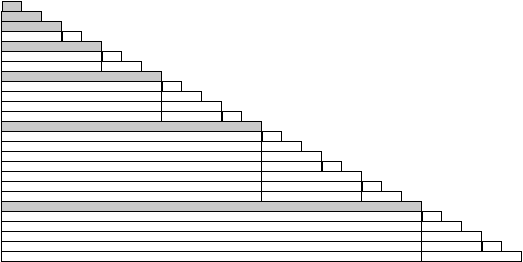
\includegraphics[scale=0.5]{FiguresArithmetic/Zeckendorf}
        \caption{The first $26$ integers (on the vertical [Y] axis), represented in the Zeckendorf system.  The breaks in the horizontal bars represent the summations of Fibonacci numbers.  The shaded horizontal bars correspond to pure Fibonacci numbers.}
\label{fig:zeckendorf}
\end{center}
\end{figure}

\subsection{A Proof of Zeckendorf's Theorem}
\label{sec:Zeckendorf-proof}

Our proof accomplishes three goals simultaneously:
\begin{itemize}
\item
It specifies an algorithm for constructing a Zeckendorf representation of every integer $n$.
\item
It verifies that the resulting representation is
  \begin{itemize}
  \item
{\em valid}---the Fibonacci numbers in the representation do, indeed, sum to $n$
  \item
{\em unique}---no other selection of Fibonacci numbers that satisfy Proposition~\ref{thm:Zeckendorf} yields numbers that sum to $n$.
  \end{itemize}
\end{itemize}
A single induction on $n$ accomplishes all three goals.  Keep in mind our nonstandard indexing of the Fibonacci sequence as you read the proof.

\medskip

\noindent {\sf Base cases}.
The Proposition holds for the cases $n=2$, $n=3$, and $n=4$.  To wit:
\[ \begin{array}{l}
F(3) \ = \ 2 \\
F(4) \ = \ 3 \\
F(4) + F(2) \ = \ 3 + 1 \ = \ 4
\end{array}
\]
Uniqueness, which asserts that no other sum of Fibonacci numbers that satisfy the Proposition yield the indicated values, is left as an exercise.

\medskip

\noindent {\sf Inductive hypothesis}.
Assume for induction that any integer $m < F(r)$ admits a unique representation of the form specified in Proposition~\ref{thm:Zeckendorf}.

\medskip

\noindent {\sf Inductive extension}.
Focus on an arbitrary integer $n$ in the interval
\[ [F(r) \leq n < F(r+1)] \]
We claim that every $n$ in this interval admits a unique Zeckendorf representation.

\smallskip

Of course, this claim is true for the smallest $n$ in the interval, namely, $n=F(r)$, because the equation ``$n=F(r)$" obviously specifies a valid Zeckendorf representation of $n$.  (We leave it to the reader to verify that this representation is unique.)

\smallskip

Focus, therefore, on an arbitrary $n \neq F(r)$ within the interval.  Write this $n$ in the form $n = F(r) + m$.  Note that we must have $m < F(r)$, by specification of the interval and by the defining recurrence of the Fibonacci sequence.  Consequently, our inductive hypothesis tells us that the integer $m$ admits a unique Zeckendorf representation:

\hspace*{.25in} $m \ = \ F(k_1) \ + \ F(k_2) \ + \cdots + \ F(k_\ell)$

\smallskip

\noindent
where \ \ $k_1 \ \gg \ k_2 \ \gg \cdots \gg \ k_\ell \ \geq \ 2$.

\smallskip

\noindent
This means that the integer $n$ admits a representation of the form

\hspace*{.25in} $n \ = \ F(r) \ + \ F(k_1) \ + \ F(k_2) \ + \cdots + \ F(k_\ell)$

\smallskip

\noindent
where \ \ $k_1 \ \gg \ k_2 \ \gg \cdots \gg \ k_\ell \ \geq \ 2$.

\smallskip 

Our final task is to verify that $F(r)$ and $F(k_1)$ are not consecutive Fibonacci numbers, or equivalently, to verify that $F(k) \gg F(k_1)$.  To this end, assume, for contradiction, that $k_1=r-1$.  Were this the case, we would have (from the Fibonacci recurrence)
\[ n \ = \ F(r+1) \ + \ F(k_2) \ + \cdots + \ F(k_\ell) \]
This equality would contradict the fact that $n < F(r+1)$.

\smallskip

This argument verifies the uniqueness as well as the validity of $n$'s Zeckendorf representation.

\medskip

Our inductive proof yields an effective way to compute the Zeckendorf representation of any number $n$---but here are likely more efficient conversion procedures.

\subsection{Zeckendorf Representations as a Number System}
\label{sec:Zeck-rep-number-system}

\index{Fibonacci number system}
One can employ Zeckendorf representations as a numbering system for positive integers:  As we just showed, each $n \in \N^+$ admits a unique such representation; we can expand the system to the set $\N$ by explicitly appending the number $0$ to the system.  This section discusses some of the pros and cons of the resulting system.

\index{Fibonacci number system!numerals}

\subsubsection{The system's numerals}

The natural way to represent numerals within the Fibonacci number system is as bit-strings.  We employ a somewhat strange system of indexing in order to be consistent with the notation of Proposition~\ref{thm:Zeckendorf}.
\begin{itemize}
\item
$0$ is the unique numeral for the number $0$.
\item
For all {\em positive} integers $n$: Each length-$\ell$ bit-string
\[ b_{\ell+1} b_{\ell} \cdots b_2 \]
where each $b_i \in \{0,1\}$, is the unique numeral for the positive integer
\[ n \ = \ (b_{\ell+1} b_\ell \cdots b_2)_F \ \eqdef \  \sum_{k=2}^{\ell+1} \ b_k \cdot F(k) \]
\end{itemize}
%Note: we wrote here the representation of $n$ in the Fibonacci numbering system using parenthesis in order to avoid confusions on the indices.

\subsubsection{Observations about the system's numerals}

We offer a few comparisons between the numerals of the Fibonacci number system and those of the binary (base-$2$) number system.

\smallskip

The first thing we notice is that base-$2$ numerals are often shorter than Fibonacci numerals. The integer $12345$ provides an illustrative example.  The {\em shortest} Fibonacci numeral for $12345$---i.e., the numeral with no leading $0$s---is the $21$-bit string
\[ 12345 \ = \ 1 00001 01000 01000 00010_F \]
The corresponding base-$2$ numeral has only $13$ bits:
\[ 12345 \ = \ 110 00001 11001_2 \]

\medskip

A second observation is that Fibonacci numerals never have consecutive $1$s.  This feature endows the Fibonacci system with a modicum of {\em error detectability}---cf., \cite{PetersonW81}---which can be a significant, {\em positive} practical attribute.

\index{error detecting codes}

\medskip

One can get a better perspective on numeral lengths and on the impact of not allowing consecutive $1$s by perusing Table~\ref{tab:FIBO1-15}.

\begin{table}[htb]
\caption{Comparing the base-$2$ and Fibonacci numerals for integers $1$--$15$}
\label{tab:FIBO1-15}
\begin{tabular}{|rclclcl|}
\hline
$n$ & & Base-$2$  & & Fibonacci  & & Relevant Fibonacci numbers \\
       & & ($4$-bit)    & & ($5$-bit)   & & \\
\hline
\hline
$1$ & & $0001_2$ & & $00001_F$ & & $F(2) =1$ \\
\hline
$2$ & & $0010_2$ & & $00010_F$ & & $F(3) = 2$ \\
\hline
$3$ & & $0011_2$ & &  $00100_F$ & & $F(4) = 3$ \\
\hline
$4$ & & $0100_2$ & &  $00101_F$ & & $F(4) + F(2) = 3+1$ \\ 
\hline
$5$ & & $0101_2$ & &  $01000_F$ & & $F(5) = 5$ \\
\hline
$6$ & & $0110_2$ & &  $01001_F$ & & $F(5) + F(2) = 4+1$ \\
\hline 
$7$ & & $0111_2$ & &  $01010_F$ & &  $F(5) + F(3) = 5+2$ \\
\hline 
$8$ & & $1000_2$ & & $10000_F$ & &  $F(6) = 8$ \\ 
\hline
$9$ & & $1001_2$ & & $10001_F$ & &  $F(6) + F(2) = 8 +1$ \\ 
\hline
$10$ & & $1010_2$ & & $10010_F$ & &  $F(6) + F(3) = 8 +2$ \\ 
\hline
$11$ & & $1011_2$ & & $10100_F$ & &  $F(6) + F(4) = 8 +3$ \\ 
\hline
$12$ & & $1100_2$ & & $10101_F$ & &  $F(6) + F(4) + F(2) = 8 +3 +1$ \\ 
\hline
$13$ & & $1101_2$ & & $10000_F$ & &  $F(7) = 13$ \\ 
\hline
$14$ & & $1110_2$ & & $10001_F$ & &  $F(7)  + F(2) = 13 +1$ \\ 
\hline
$15$ & & $1111_2$ & & $10010_F$ & &  $F(7) + F(3) = 13 +2$ \\ 
\hline
\end{tabular}
\end{table}
 
\subsubsection{On incrementing Fibonacci numerals}

Our final look at the Fibonacci system illustrates how differently the system's numerals behave  when being manipulated, as compared with the numerals from positional number systems.  We describe a procedure for {\em incrementing} numbers---i.e., adding $1$---within the Fibonacci system.  Of course, one must employ ever-longer Fibonacci numerals as one deals with ever-larger numbers---a simple consequence of the Pigeonhole Principle.\footnote{The Principle asserts that only finitely many numbers can be represented by numerals of any fixed length.}  It is interesting to observe how the {\em carries} that embody the lengthening of numerals reflect the underlying Fibonacci recurrences---and to compare this process with the way carries operate within standard positional number systems (which the reader learned in elementary school).

\index{Fibonacci number system!carries}
\index{Fibonacci number system!incrementing numerals}
\index{Fibonacci number system!incrementing integers}

\smallskip

\noindent
For the sake of precision, what we shall present is a procedure that transforms a Fibonacci-system numeral
\[ a_n a_{n-1} \cdots a_1 a_0 \]
that denotes the integer
\[ (a_n a_{n-1} \cdots a_1 a_0)_F \]
to a Fibonacci-system numeral
\[ b_m b_{m-1} \cdots b_1 b_0 \]
that denotes the integer
\[ (b_m b_{m-1} \cdots b_1 b_0)_F \ = \ 1 \ + \ (a_n a_{n-1} \cdots a_1 a_0)_F \]

Perhaps the simplest procedure for achieving this transformation---and achieving it {\em efficiently}---relies on the system of equations (\ref{eq:multilinear-Fib-2}) from Proposition~\ref{thm:FiboSum-2}.  We repeat the system for the reader's convenience:

\medskip

\noindent For all integers $n \geq 2$,
\[
F(n) \ \ = \ \
F(n-1) \ + \ F(n-3) \ + \ F(n-5) \ + \cdots + \ 1
\]

\medskip

By combining this system with the fact that the Fibonacci system prominently avoids consecutive $1$s in numerals, one verifies that the procedure we describe now correctly computes the {\em increment} operation.  Let us begin with the input Fibonacci-system numeral
\[ \alpha \ = \  a_n a_{n-1} \cdots a_1 \]

\bigskip

\noindent {\bf Procedure} {\em INCREMENT}($\alpha$) \\
{\bf begin}
\begin{description}
\item[{\sf Step} 1]
Prepend two consecutive $0$s to $\alpha$, to produce the bit-string
\[  \alpha^{(00)} \ \eqdef \  0 0 a_n a_{n-1} \cdots a_1 \]

\item[{\sf Step} 2]
Find the {\em rightmost} consecutive positions in $\alpha^{(00)}$ that contain two consecutive $0$s.  Say that the portion of $\alpha^{(00)}$ beginning with the discovered two consecutive $0$s and proceeding rightward from there has the form
\[  \alpha^{(right)} \ \eqdef \  0 0 a_\ell a_{\ell-1} \cdots a_1 \]
Because of our prepending step, index $\ell$ will always exist---i.e., the search will always succeed.   Index $\ell$ will be smaller than index $n$ precisely if the input numeral $\alpha$ contains two consecutive $0$s (in one or more places).

\item[{\sf Step} 3]
Replace the bit-string $\alpha^{(right)}$ within the numeral $\alpha$ by the bit-string
\[ 0 1 0 0 \cdots 0 \ \ \ \mbox{ ($n$ terminal $0$s)} \]
\end{description}
\noindent {\bf end} {\em increment} procedure

\bigskip

\noindent We extract two illustrations from Table~\ref{tab:FIBO1-15}:
\[ \begin{array}{ccrcrcccrcr}
n_1 & = & 7 & = & 1010_F & \hspace*{.25in} & 
     \mbox{incr}(n_1) & = & 8 & = & 10000_F  \\ 
n_2 & = & 9 & = & 10001_F & \hspace*{.25in} &
     \mbox{incr}(n_2 ) & = & 10 &  = &10010_F
\end{array}
\]

\bigskip

We leave to the reader the exercise of extending our incrementation procedure to devise an algorithm for performing general additions within the Fibonacci system.


